\documentclass[letterpaper, 12pt]{article}
\title{CSE471 - Homework 3}
\author{Kumal Patel}
\date{\today}

\usepackage{float, graphicx, amssymb}


\begin{document}   
\maketitle

\begin{enumerate}
    \item[Exercise 1.1] 
    \begin{enumerate}
        
        \item Applying alpha-beta pruning figure 1 \\
        \begin{figure}[H]
            \centering
            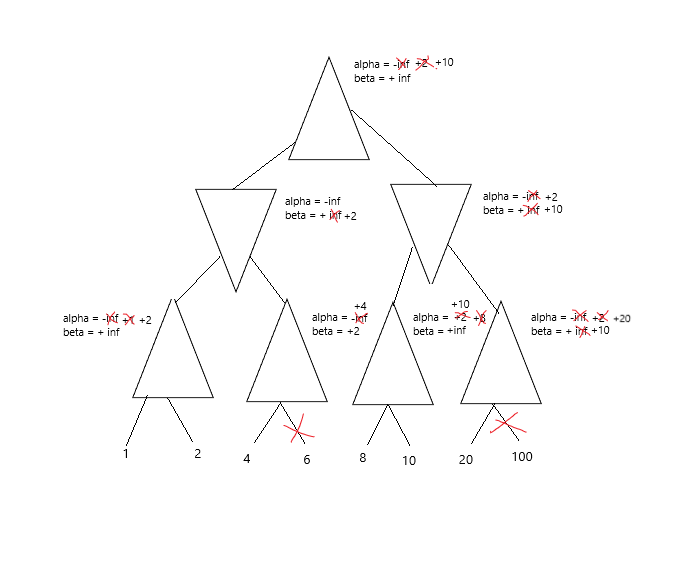
\includegraphics[width=\linewidth]{q1.a.png}
            \caption{Shows alpha-beta values at each node}
        \end{figure}

        \item Applying alpha-beta pruning figure 2 \\
        \begin{figure}[H]
            \centering
            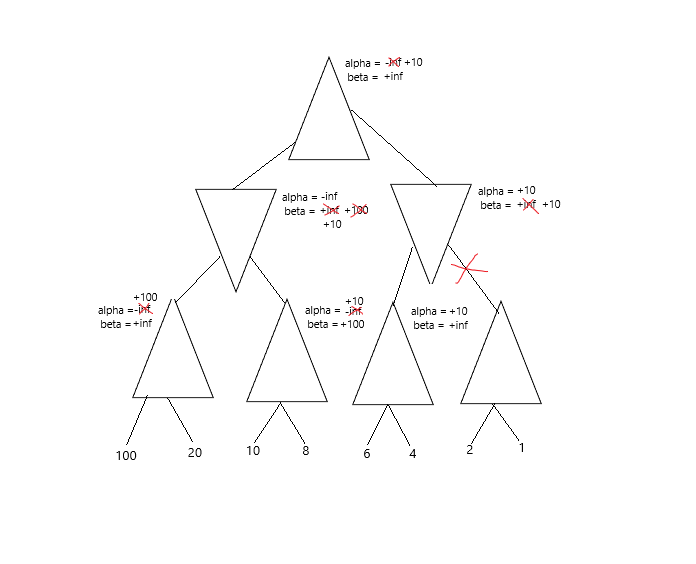
\includegraphics[width=\linewidth]{q1.b.png}
            \caption{Shows alpha-beta values at each node}
        \end{figure} 

        \item Applying alpha-beta pruning figure 3 \\ \\The ordering of the leaf nodes matter. 
            Pruning occurs when alpha $\geq$ beta. So at f and g (at node 100 and 8), $alpha=-\infty$ and $beta=10$.
            Since the first leaf node is 100, and $100\geq10$, we prune. But if 8 was the first leaf
            it would not prune because $8\ngeq10$.
        \begin{figure}[H]
            \centering
            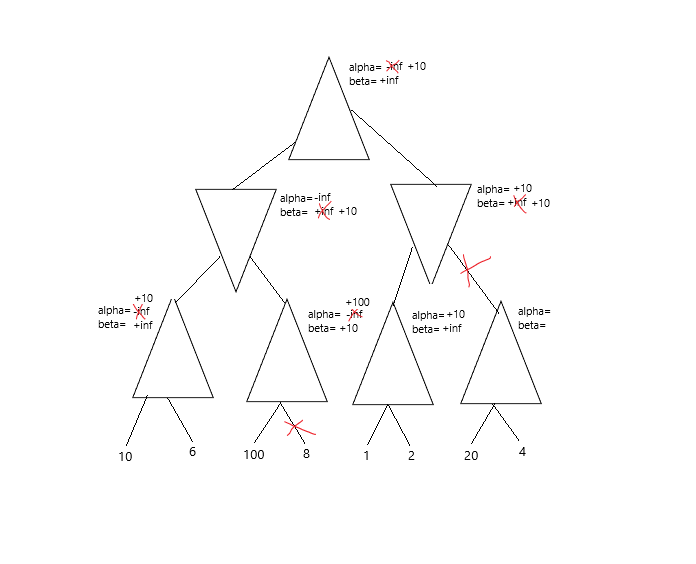
\includegraphics[width=\linewidth]{q1.c.png}
            \caption{Shows alpha-beta values at each node}
        \end{figure} 
        
    \end{enumerate} 
    \item[Exercise 1.2]  
    \begin{enumerate}
        \item To ensure X1 and its leaf nodes will not be pruned $A,B,C$ can be $8,8,500$.
            Since the max node above X1 has an alpha value of 7. To ensure X1 doesn't prune
            beta would need to be greater than 7. The value of beta is determined from A or B.
            And lastly, at node X1, C would need to be greater than A and B to ensure beta is greater
            than alpha. Choosing a large number like 500 for example would work.
        \item At node n1 to prune $A,B,C$ can be $8,8,5$. The values of A and B can remain the same
            from part a. C on the other has to be less than or equal to 7 to prune. Since the value 
            of alpha at node X1 is 7.
        \item At node n2 to prune $A,B,C$ can be $5,5,500$. The value of C can remain the same from part a.
            A or B on the other hand has to be greater than or equal to 0 to prune. Since the leaf node is 0, 
            beta becomes 0, and the value of alpha would need to be greater or equal to 0 to prune.
    \end{enumerate} 
    \item[Exercise 1.3] 
    \begin{enumerate}
        \item When the leaf values are finite and unbounded pruning is not possible in a max tree.
            Because the other branch may contain a higher leaf value than the leaf value that was visited before.
        \item Pruning is not possible under the same conditions because for the same reasons as A. The expectimax node
            must be computed entirely as well for the max node above.
        \item If the leaf values are all nonnegative, pruning is not possible in a max tree. Because the root value of a max tree is the best leaf value. 
        And any unvisited leaf value may be the best leaf value, so therefore, all the leaves must be seen.
        \item Pruning is not possible in a expectimax tree when all the leaf values are nonnegative. 
            Because the nonnegative values show the lower bound of the chance node. Since pruning is not allowed on the lower bound, pruning is not possible.        
        \item If the leaf values are in the range of [0,1] it can be pruned in a max tree.
        \begin{figure}[H]
            \centering
            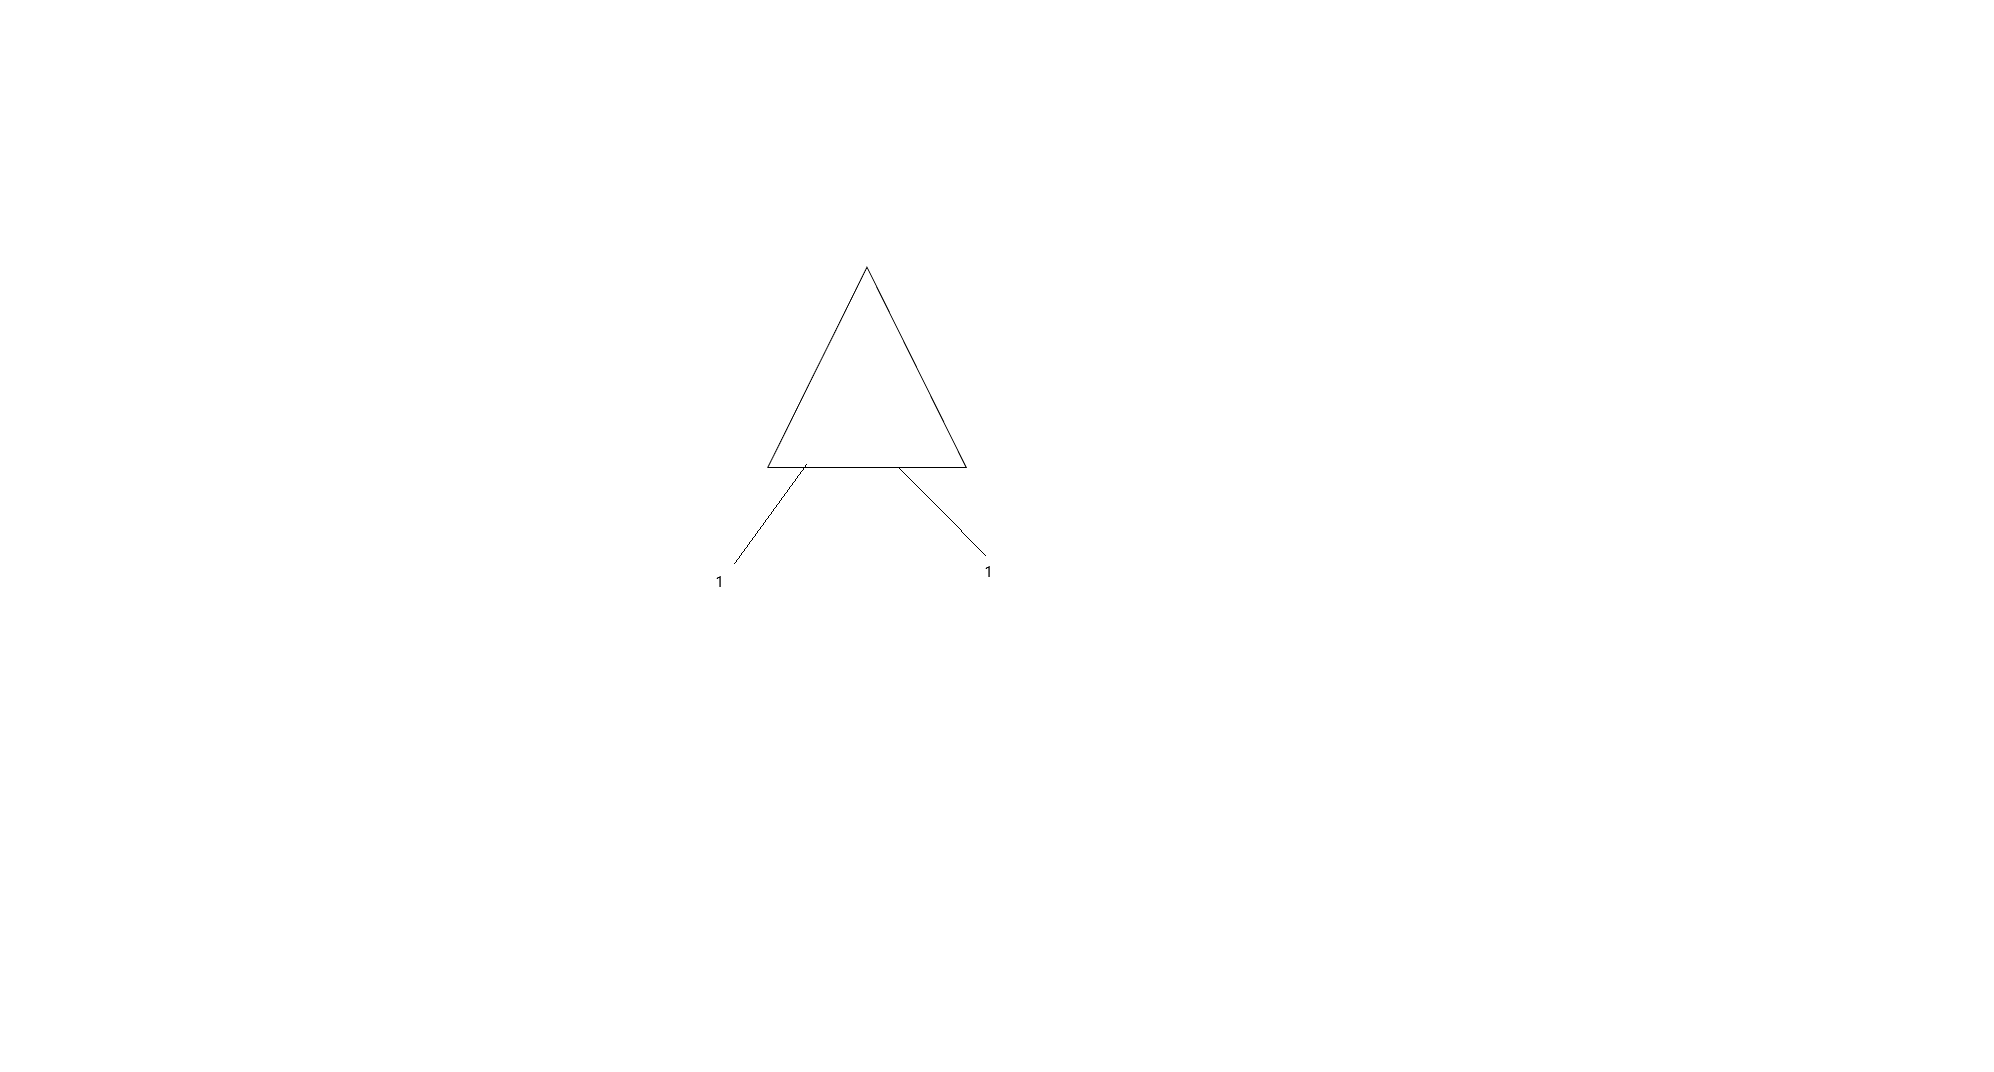
\includegraphics[width=.8\linewidth]{q3.e.png}
            \caption{Example showing that the second leaf can be pruned}
        \end{figure} 
        \item If the leave values are in the range of [0,1] it can be pruned in an expectimax tree.
        \begin{figure}[H]
            \centering
            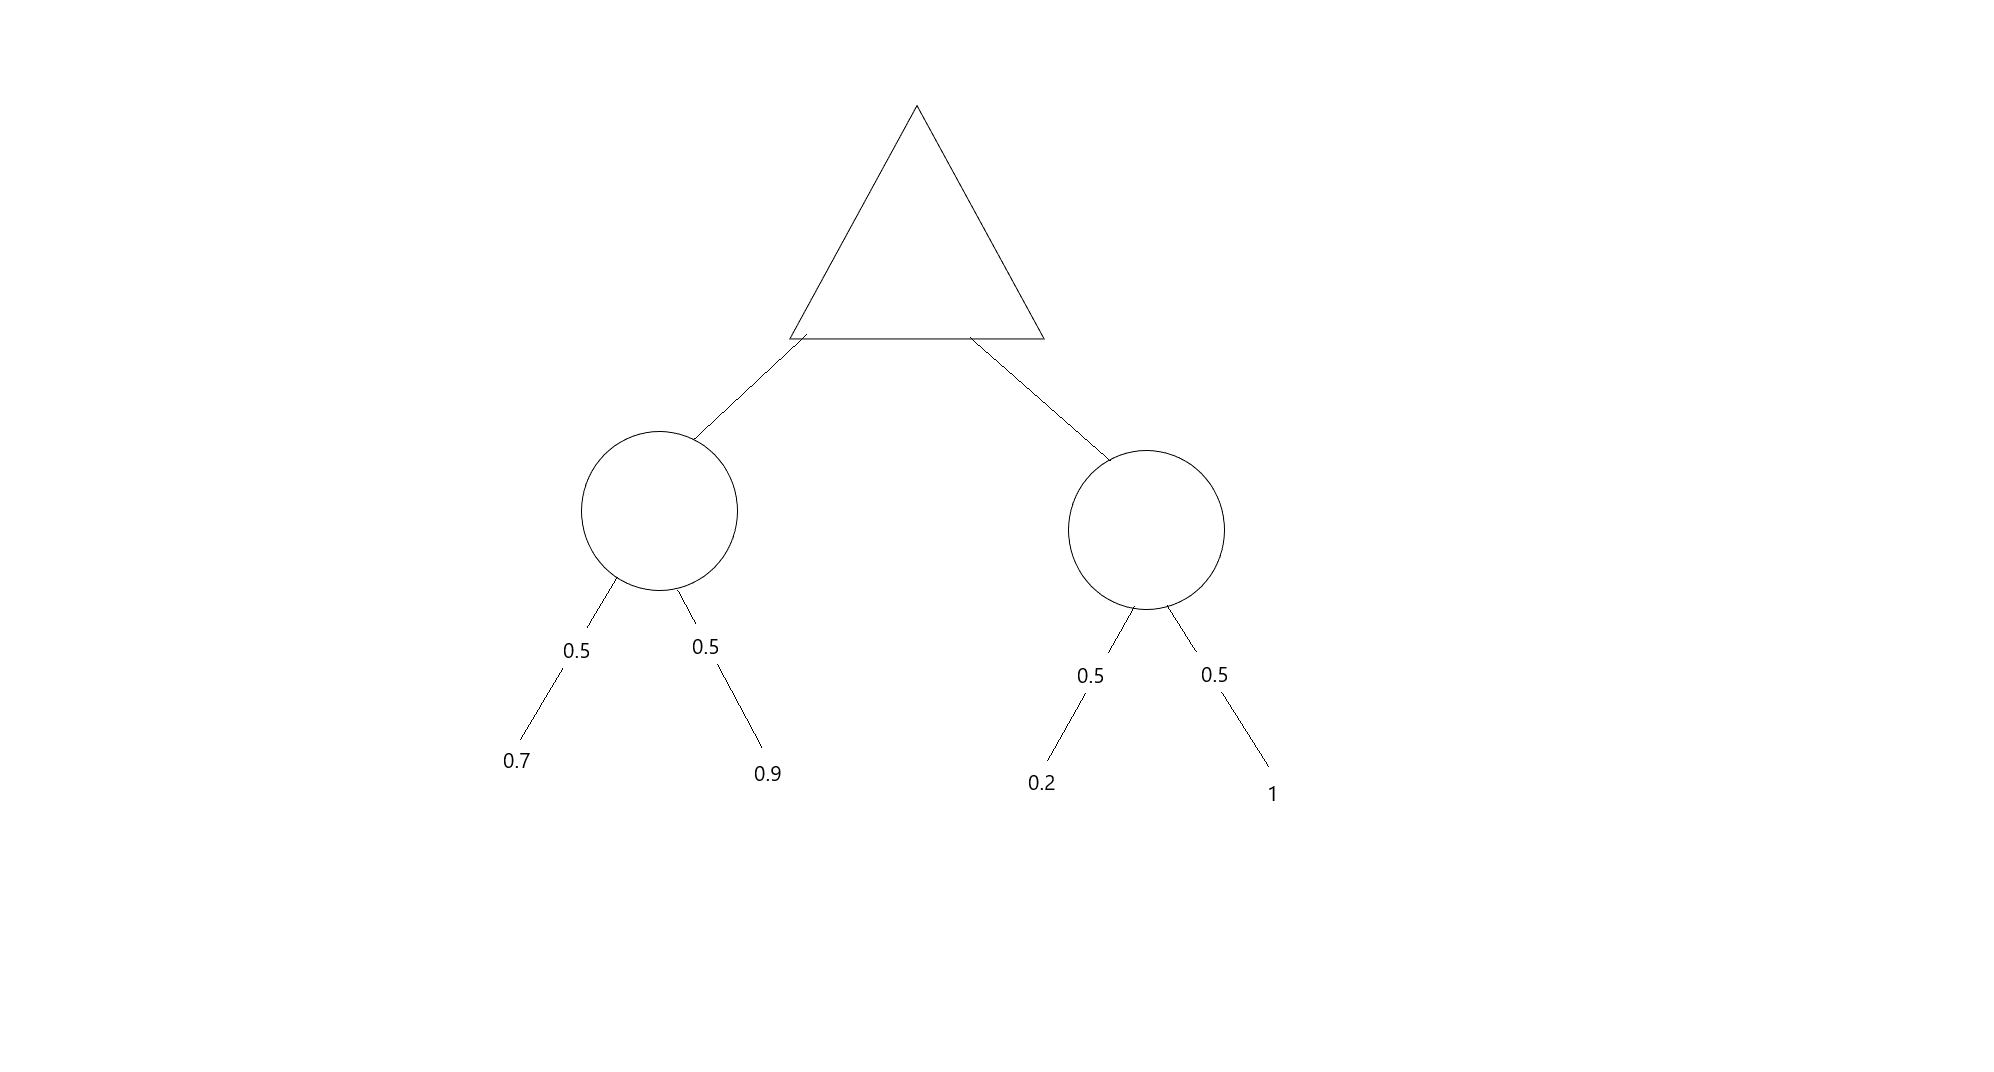
\includegraphics[width=.8\linewidth]{q3.f.png}
            \caption{Example showing that the right most leaf can be pruned}
        \end{figure} 
        \item The highest probability first evaluation order is most likely to yield when pruning.
            Because this makes the strongest bound on the value of the node. 
        
    \end{enumerate}
    \item[Exercise 1.4]
    \begin{enumerate}
        \item \[ \sum_{i=0}^{M} U_i(s)=C \]
        \item \[ \sum_{i=0}^{M} -C*U_i(s) \] \[ \sum_{i=0}^{M} C*U_i(s) \]
        \item \[ \sum_{i=0}^{M/2} U_i(s)  = \sum_{M/2+1}^{M} U_i(s) \]          
    \end{enumerate}   
    \item[Exercise 1.5]
    \begin{enumerate}
        \item False, in a zero-sum game with two perfectly rational players, the players 
            would have the perfect knowledge of the game and environment. And in a fully observable 
            environment the player always knows what state it is in. So therefore, knowing all of this
            helps the first player to be able to predict the second players strategy after making its move.
        \item True, in a partially observable environment the player does not know which state it is in. And without 
            further information about the environment it would be difficult to predict the move from the second player. 
            So knowing the second players move would not help in this case.
        \item False, even though this agent is perfectly rational it may fail in some unlucky cases.
            When two agents that are perfectly rational and are playing against each other one must lose, so
            therefore it is false that a perfectly rational pacman never loses.
    \end{enumerate} 
\end{enumerate}
\end{document}